\section{\textbf{Applications with AME}}

\subsection{Design}

We apply AME to five recent IR studies: \citet{reiter:stam:2003, mcdonald:2004,  rose:2004, weeks:2012, gibler:2017}. Each of these studies are representative of broader trends in the field in that they use relational data of state interactions and propose both dyadic, monadic, and structural explanations for behavior of actors in the system. We choose to demonstrate the capabilities of AME with reference to existing studies in order to highlight several features of the AME approach. First, the results of AME estimation are interpretable alongside results using standard approaches, but, as shown in the simulation section, have the additional benefit of being able to take into account dependencies that may complicate inference. Second, through using this approach, we can also quantify the degree to which first, second, and third order dependencies are present in events of interest. Third, we show that by using the AME framework scholars can better model the data generating process behind their events of interest.

We obtained the data for each of these studies from their replication archives and replicated the main results of each article.\footnote{Without exception this was straightforward to accomplish, thanks to the authors' transparency and an increasing norm in the social sciences of open data sharing.} The five studies used below were selected based on how recent they were and whether they had more then 100 citations.\footnote{Note that we chose papers with at least 100 citations as an indicator of influence within the discipline. Of course, by the criteria of influence many other papers could have been considered for the replication. However, as described in the following sections, the AME model has specific data requirements, which limited the scope of potential papers.} Each of these pieces, published in prominent journals well-known in their respective literatures, posited a theory in which interdependencies are consequential. Reflecting the dominant approach in the literature, each of the authors tested their hypothesis by employing some form of a general linearized model.\footnote{It is important to note that the AME framework is applicable only where a full set of dyads for an outcome of interest is observable---for example it is unsuitable for studying onsets, where dyad-years representing conflict continuations are removed from the sample. The AME is also not applicable to analyses of case-level data, for example, studies that examine the decision to go to war by particular states.}

\begin{table}
\caption{Features of the Studies Re-estimated.}
	\begin{tabular}{lcccccc}
		& Model &  Date Range & N. Actors  & N. Dyads & Dyads Type & Clustering $\sigma_{\hat{\beta}}$ \\ \toprule
		Reiter \& Stam (2003) &Logit &1945--1995 &  193 & $753,456$ & Directed & Robust \\	
		McDonald (2004) & Logit &1959--2002 & 198 & $92,354$ & Undirected & Robust\\
		Rose (2004) & OLS & 1948--1999 & 177 & $234,597$ & Directed & Robust \\	 
		Weeks (2012) & Logit & 1946--1999 &197 &  $901,540$ & Directed & Robust \\
		Gibler (2017) & Logit & 1816--2008 &193 &   $650,557$ & Undirected & None \\ \bottomrule
	\end{tabular}
\end{table}

Each of the five studies has a crucial finding that we hone in on to further draw into focus the analytical power of the AME estimation procedure.  In Table~\ref{tab:modelFindingSumm}, we present the overall results; the term \textit{Unconfirmed} indicates only that the sign and/or significance of the putatively crucial finding in the original study is not found to hold in the AME estimation.\footnote{Full tabular results for each of the original and reestimated models are presented in the Appendix.}

\begin{table}[ht]
\centering
\caption{Here we provide a brief summary of the key variable in each of the five replications and a note about whether or not the highlighted finding remains when using our network-based approach.}
	\begin{tabular}{l p{7cm} l} \toprule
		\multirow{2}{*}{Study} & \multirow{2}{*}{Central Finding} &  Confirmed \\
		& &  accounting for dependencies? \\ \toprule
		Reiter \& Stam (2003) & Personalist Regimes Attack Democracies, Not Vice Versa & {Partially Confirmed} \\ \midrule
		McDonald (2004) & Lower Trade Barriers and Higher Trade Lead to Peace & {Unconfirmed}\\ \midrule
		Rose (2004) & WTO Membership Does not Affect Trade & {Partially Confirmed}\\ \midrule
		Weeks (2012) & Bosses, Juntas, and Strongmen are more Aggressive, Machines are Not & {Unconfirmed} \\\midrule
		Gibler (2017) & Power Parity at Time of Entry to International System Inceases Conflict & {Unconfirmed}\\ \bottomrule
	\end{tabular}
	\label{tab:modelFindingSumm}
\end{table}

An important takeaway here is that many scholars are forced to make knowledge claims based on the statistical significance of a small set of covariates, or the differences between these covariates. These differences may change dramatically when interdependencies are taken into account directly, as they do in the case of this study. This outcome follows from AME's ability to better account for the dependencies discussed in the previous section, whereas GLM approaches explicitly assume observational independence conditional on the specified covariates. As this is a widely-known limitation of GLM approaches, scholars often attempt to account for clustering of observations by including additional variables and adjusting the standard errors of the resulting estimates. At best, this method introduces noise and imprecision into results, and at worst can produce misleading outcomes. Beyond just comparing parameter estimates, we examine how well each approach can represent the data generating process using an out-of-sample cross validation strategy. Specifically, for each study, we randomly divide the data into $k=30$ sets, letting $s_{ij,t}$ be the set to which pair $ij,t$ is assigned.

Then for each $s \in \{1,\ldots,k\}$, we:

\begin{enumerate}
	\item estimate model parameters with $\{y_{ij,t}: s_{ij,t} \neq s\}$, the data not in set $s$,
	\item and predict $\{\hat{y}_{ij,t}: s_{ij,t} = s\}$ from these estimated parameters. 
\end{enumerate}

The result of this procedure is a set of sociomatrices $\bm \hat Y$, in which each entry $\hat y_{ij,t}$ is a predicted value obtained from using a subset of the data that does not include $y_{ij,t}$.\footnote{For more details on this type of cross-validation strategy see \citet{minhas:etal:2016:arxiv}.} We summarize the performance of the various models in Table~\ref{tab:modelPerfSumm} below. For the binary models we  provide the area under the Receiver Operator Characteristic (ROC) and Precision Recall (PR) curves. Only one of the studies here had a continuous dependent variable and for this we provide the root mean squared error (RMSE) and root median squared error (RMDSE).\footnote{More details on the performance of each of these models can be found in the Appendix.} For each of the replications, we find that the AME approach substantially outperforms the original models in terms of out-of-sample predictive performance.

\begin{table}[ht]
\centering
	\begin{tabular}{l|l cc}
	~ & ~ & GLM & AME \\
	\toprule
		\multirow{2}{*}{Reiter \& Stam (2003)} & Area Under ROC Curve, AUC-ROC & 0.92 & {0.96} \\
				~ & Area Under PR Curve, AUC-PR & 0.08 &  {0.15} \\		\midrule
		\multirow{2}{*}{McDonald (2004)} & AUC-ROC & 0.92 &  {0.99} \\
				~ & AUC-PR & 0.13 &  {0.28} \\		\midrule
		\multirow{2}{*}{Rose (2004)} & RMSE & 3.23 &  {1.99} \\
				~ & RMDSE & 2.01 &  {1.06} \\	\midrule
		\multirow{2}{*}{Weeks (2012)} & AUC-ROC & 0.64 &  {0.97} \\
				~ & AUC-PR & 0.00 &  {0.15} \\		\midrule
		\multirow{2}{*}{Gibler (2017)} & AUC-ROC & 0.52 &  {0.91} \\
				~ & AUC-PR & 0.00 &  {0.08} \\			\bottomrule
	\end{tabular}
	\caption{Here we provide a summary of the out-of-sample performance based on our cross-validation strategy for each of the five replications when using the standard dyadic approach and our network-based approach. Four of the five studies involved a binary dependent variable; for those measures, area under the curve (AUC) statistics are reported. The Rose study involved a Gaussian dependent variable and for that we use the root mean squared error (RMSE) and root median squared error (RMDSE). 
	}
	\label{tab:modelPerfSumm}
\end{table}
\FloatBarrier

Next we discuss each of the replications in more detail and highlight the substantive insights that can be drawn from the AME framework.

\subsection{Re-estimation of Reiter \& Stam (2003)}

\citet{reiter:stam:2003} examine the relationship between democracy, dictatorship and the initiation of militarized disputes. Their work contests prior scholarship that had claimed interstate dyads containing democracies and personalist dictatorships were particularly prone to conflict because of aggression on the part of the democratic state. Using directed dyads, they find evidence against this hypothesis: dictators are in fact more likely to challenge democracies, but not the other way around.  In addition, military regimes and single-party regimes are more prone to initiate disputes with democracies, but the opposite is not true. Independent variables focus on various encodings of regime types, contiguity, alliance, and capability measures. As is prevalent in this literature, Reiter \& Stam employ a logistic regression that includes an indicator of the time since the last dispute as well as three cubic splines. The database for this study is constructed using \texttt{EUGene} \citep{bennett:stam:2000} and comprises approximately three-quarters of a million stacked dyads. Based on their statistical analysis, they conclude that institutional constraints affect the propensity of democratic and non-democratic leaders to engage in military conflict. 

In the original model, the variable ``Pers/Democ Directed Dyad" (which represents a Personalist $\rightarrow$ Democractic directed dyad) has a positive effect while the variable ``Democ/Personalist Directed Dyad'' is too imprecisely measured to indicate a direction. In our re-estimation using the AME framework, we also find that Pers-Democ directed dyad has a positive effect while Democ-Pers directed dyad is still too imprecisely measured to indicate a direction. Using this model, however, we can no longer conclusively say that the Pers/Democratic coefficient is larger than the Democ/Personalist one. Our re-estimation using the AME approach therefore cast some doubt on Reiter \& Stam's key claim that MIDs initiated by personalist dictatorships against democracies are more likely than MIDS initiated by democracies, though many of the major effects  uncovered by the authors remains robust when accounting for dyadic interdependencies. %Further, the effect of most of the covariates in the literature thought to predict interstate MIDs are much closer to zero when using the AME framework suggesting that some of their effects were actually the products of interdependencies. 

\subsection{Re-estimation of McDonald (2004)}

\citet{mcdonald:2004} studied whether trade promotes peace between nations. \citet[p. 547]{mcdonald:2004} introduced the argument that free trade between states ``makes conflict less likely because of its efficiency over conquest in acquiring resources\ldots''. Accordingly, he provided evidence challenging the generalized linkage between peace and trade and refined the measurement of the standard ``trade'' variable, arguing that \textit{free} trade, rather than trade alone, reduces the likelihood of conflict between states. His key hypothesis is that greater levels of protection increase the probability of interstate conflict, an argument that builds on the work of classic liberalism and connects free trade to the power of domestic audiences. \citet{mcdonald:2004} measured free trade in two ways. The first, the ``protection'' variable measures the proportion of customs revenue divided by total imports in the state that possesses the greater such ratio in each dyad. reflects the notion that larger protected sectors generate greater societal pressures resulting in pockets of support for war. This measure thus captures the score of the state in the dyad that possesses higher barriers to trade. \citet[p. 560]{mcdonald:2004} also includes a measure of economic integration  calculated as ``the lower proportion of total dyadic trade (imports plus exports) divided by state $i$'s GDP or total dyadic trade divided by state $j$'s GDP''. The (binary) dependent variable is the onset of a new militarized interstate dispute within a given dyad.  \citet{mcdonald:2004} employs logistic regression to examine the  putative statistical significance of these variables. The models  include splines to correct for temporal dependence, and robust  standard errors clustered on each dyad.

Our re-estimation with AME reveals that trade relations are highly interdependent and exhibit important patterns of transitivity.  Or, in other words, if countries $i$ and $j$ are highly dependent and countries $j$ and $k$ are also highly dependent, then we are likely to observe high dependency between countries $i$ and $k$. This indicates that conflict is less likely among members of a trade community. Once we control for these dependencies, we can more clearly interpret the positive link between trade and conflict.  The most striking thing is that AME finds a positive conditional association between trade dependence and conflict ($\hat{\beta}= 18.4, \quad \sigma_{\hat{\beta}} = 28.6$), while the comparable numbers for the logistic regression found in the original articles are negative ($\hat{\beta}= -22.2, \quad \sigma_{\hat{\beta}} = 15.2$). At the same time, the AME has ROC and PR curves (shown in the Appendix) that dominate the results found in McDonald (2004).

\subsection{Re-estimation of Rose (2004)}

\nocite{rose:2004}
In 2004, Andrew Rose published a study in the \textit{American Economic Review} that proved to be quite controversial in terms of macroeconomic trade theory and in terms of trade policy in a variety of nations. It also provoked a number of responses in the international political economy literature \citep{tomz:etal:2007}.  Rose's basic argument is that despite longstanding arguments, made by trade theorists and the World Trade Organization, that WTO membership fosters greater cooperation and thereby more trade among its members, the empirics do not bear out such claims. He uses a standard gravity model with dyadic data on bilateral merchandise trade (not services) for $175$ countries over a period of five decades. Estimating this model using OLS within many differing contexts, his conclusion is that: ``An extensive search reveals little evidence that countries joining or belonging to the GATT/WTO have different trade patters from outsiders \ldots (2004, page 98, abstract).''  The data for this study have been widely used in replications by many searching for the missing effects of the WTO---as well as preferential trade agreements, bilateral investment theories, and other aspects of modern trade theory.  

When we compare the results of Rose's original OLS model to the AME model accounting for network dependencies, the results are similar. The main result of the model---the null effect of membership in the WTO, as represented by the ``One-In" and ``Both-In" variables---does not prevail in the AME model. However, in a sense the AME result provides even stronger evidence against a positive effect of WTO membership: in the original model, this negative linkage is not significant, but in the AME estimation this negative linkage is more precisely estimated. The fact that this variable attains conventional statistical significance under an AME estimation shows an additional value of this approach to applied researchers -- while accounting for interdependencies and removing that source of bias will remove false positive findings, it can also avoid false negative findings where the bias prevented a researcher from uncovering a consistent relationship.\footnote{This benefit comes up less often in these replications because most published studies are positive, rather than null findings.} In both cases we find  a rejection of the conventional wisdom, that WTO membership increases trade. While in the original model there was a clear positive relationship between Real GDP and Trade, most of this effect vanishes in the AME model. Of course, the controversial result of the paper, strengthened in the AME analysis might be an artifact of measurement error. \citep{tomz:etal:2007}. While in the original model there was a clear positive relationship between Real GDP and Trade, most of this effect vanishes in the AME model. 

\begin{figure}
	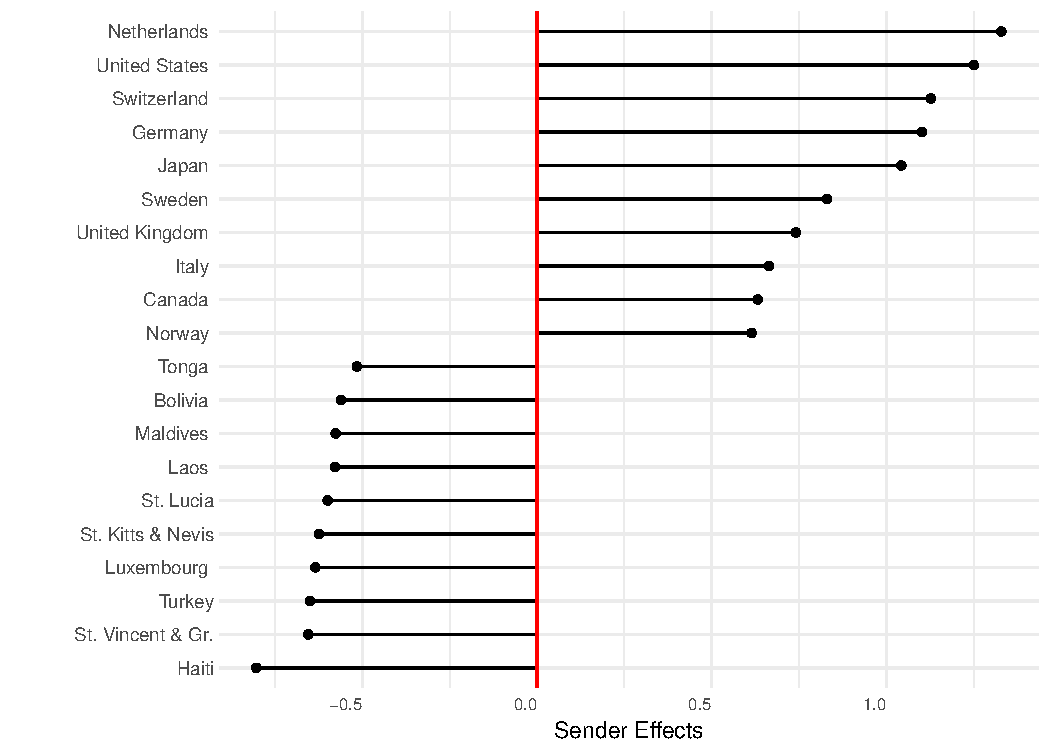
\includegraphics[width=\textwidth]{rose_aeff_top10.pdf}
	\caption{Nodal Random Effects for AME estimation of Rose (2004), for the countries with the highest and lowest Random Effects.}\label{fig:roser}
\end{figure}
\FloatBarrier

The random effects shown in Figure~\ref{fig:roser} reveal the cause of much of this divergence. Here, the states with the most positive random effects are also states with high GDP, though not necessarily high GDP/capita.\footnote{Note: Qatar exhibits strongly negative random effects.}  Most of the other results of the model are constant across each model, though some geographic features, such as islands and landlocked states, have a more clear effect on trade once we account for these network dependencies. When we account for network interdependencies, we observe a markedly lower Root Mean Squared Error out-of-sample --- $3.23$ for the OLS model and $1.77$ for the AME model. While the AME model replicates the main (null) result, there are substantial and substantive improvements gained from moving to an AME estimation.

\subsection{Re-estimation of Weeks (2012)}

\citet{weeks:2012} examines the influence of domestic institutions on the initiation of military conflicts by autocratic leaders.  She argues that in some circumstances autocrats are held accountable for their foreign policy decisions. She adds the nuance that autocratic audiences are not homogeneous. When the autocratic regime is nonmilitary, domestic audiences do not favor military actions, but in military autocracies this is not the case. Further she argues that in personalistic regimes without a military or civilian domestic audience, the leaders tend to be more likely to employ military force in their foreign policy.  To study this question, she uses a dyadic design in which the dependent variable is ``whether country A in a directed dyad initiated military conflict against country B during year t'' (page 337).  One major innovation in her study resides in the nuanced way in which she conceptualizes and codes regime type into four types: a) Machine, b) Junta, c) Boss, and d) Strongmen. She also includes a variety of putative control variables focusing on capabilities for both sides of the dyad, alliances, geography, trade dependence, regime instability, and the regime type of ``side B.'' She uses a logistic regression, but follows \citet{beck:etal:1998} and includes splines to capture temporal covariation in the dependent variable along with fixed, unit effects. The analysis is done for dyads, but is considered to be from the perspective of the actor that initiated the dispute. The basic finding is that a) juntas, boss type, and strongmen type regimes are more likely to initiate conflict than machine-type regimes (and maybe democracies) and that b) machine-type regimes are no more belligerent than democracies.   These insights are mainly emphasized in the paper by the parameter estimates depicted in Tables 1 and 2 (pages 339--340) from the paper. She argued that ignoring important nuances between different types of autocracies hinders our understanding of the initiation of military conflict by autocracies. 

\begin{figure}[!h]
	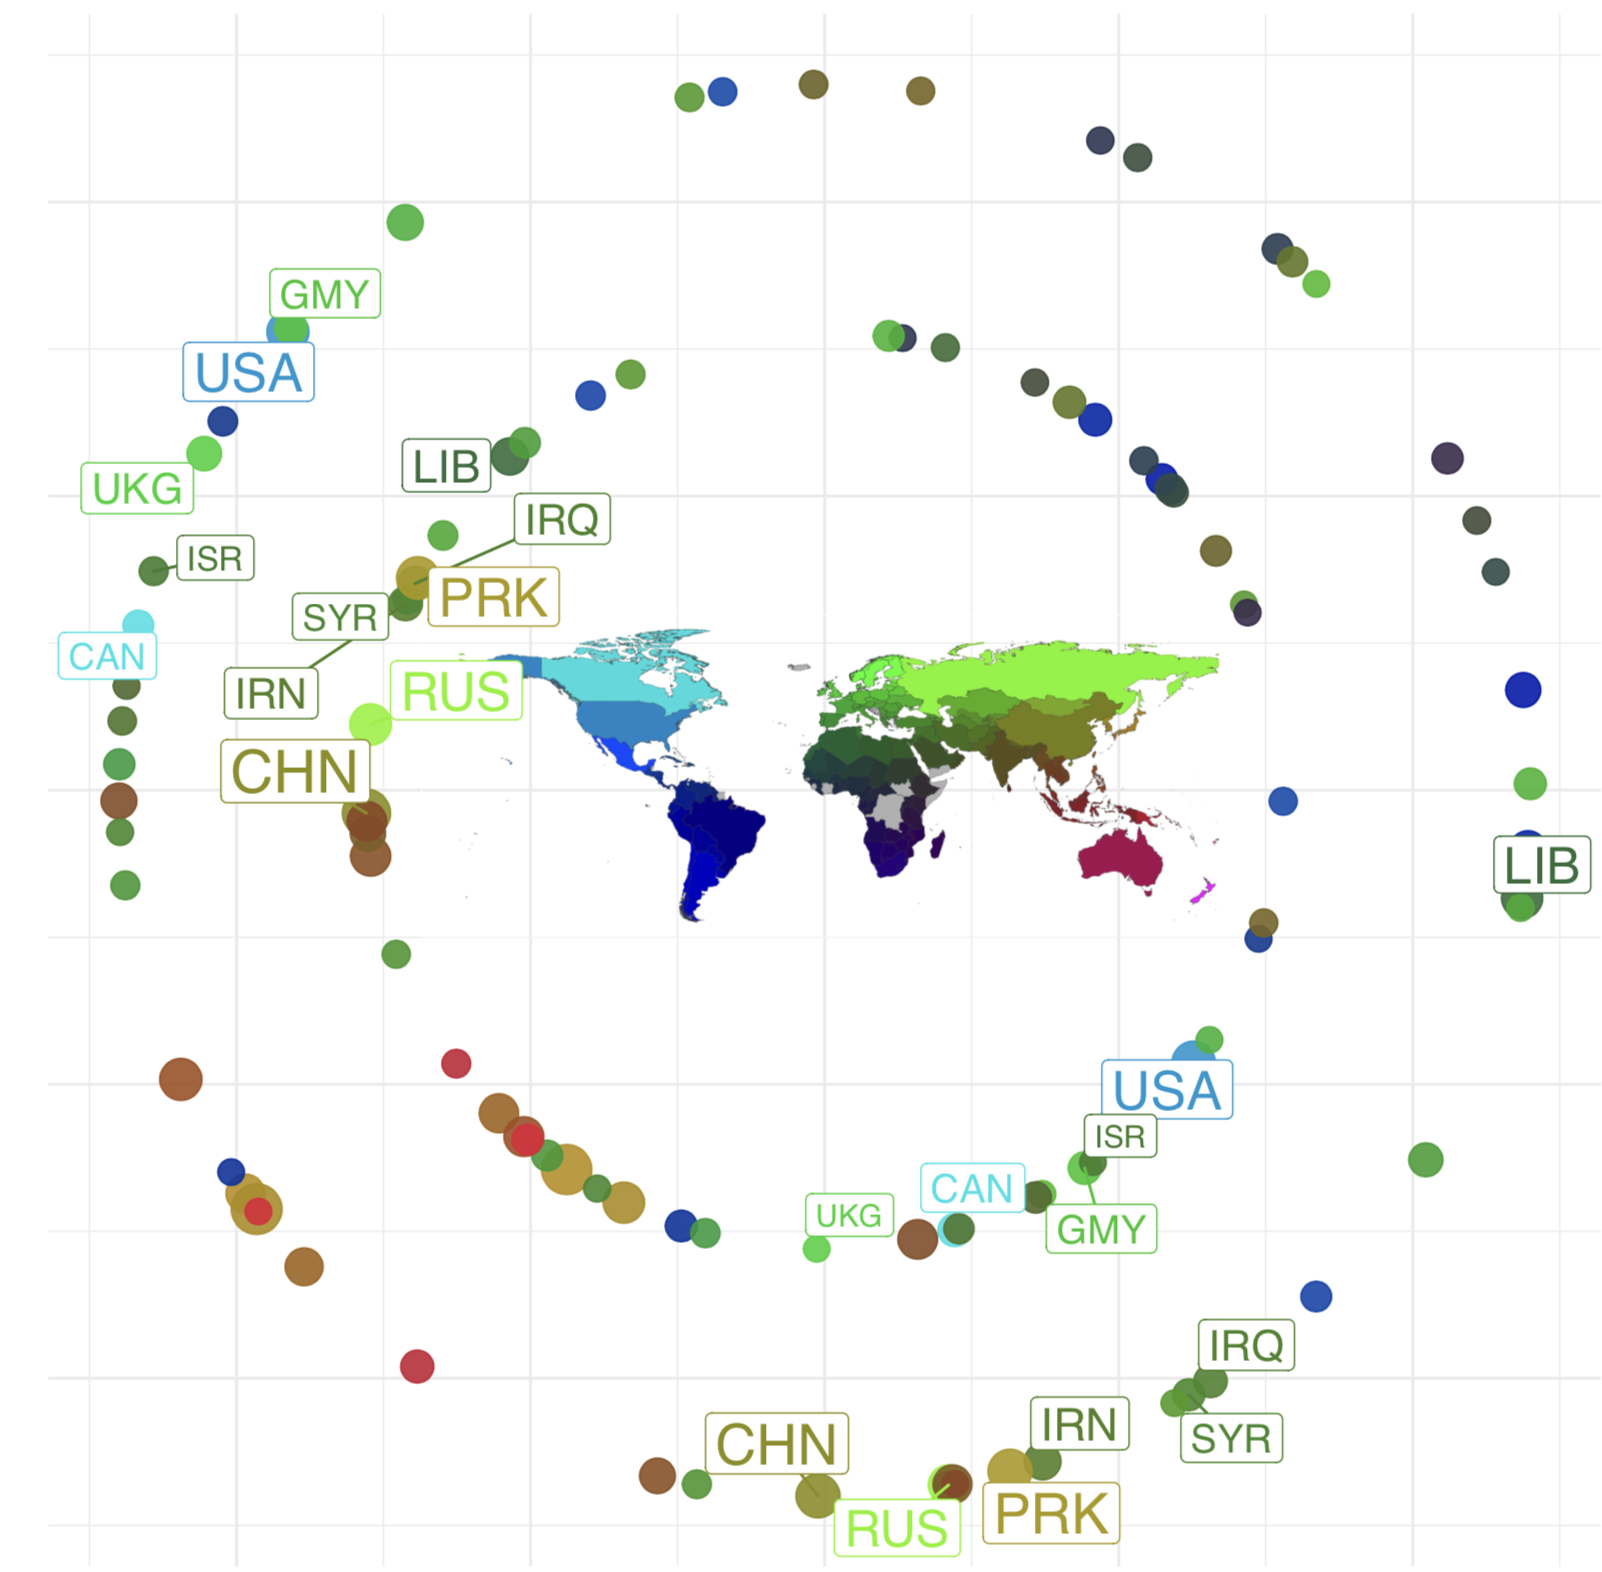
\includegraphics[width=\textwidth]{weeks_circPlot.png}
	\caption{\label{fig:weekscirc} Visualization of multiplicative effects for Weeks (2012). Each circle designates a country and the color corresponds to the legend at the center of the visualization. Countries that cluster together in the outer ring are those that were found by the model to have similar sending patterns, meaning that they tend to send conflict to similar sets of countries. The inner ring clusters countries by the similarity of who they receive conflict from. 
	%Blue represents groups with common sending patterns and red represents groups with common receiving patterns.
	}
\end{figure}
\FloatBarrier

The re-estimation of \citet{weeks:2012} has the sharpest divergence between the GLM results and those of the AME Model. In Weeks' initial models,  she finds that machines are less prone to initiate conflict than the reference category, whereas Juntas, Bosses, and Strong-men are more conflict-prone. When we examine the AME results, we find that none of these values are distinguishable from zero. Similarly, we find less pronounced effects for military capabilities. One explanation for this divergence is the AME model's ability to account for third-order effects. Inspection of the multiplicative effects in Figure~\ref{fig:weekscirc} reveals a number of clusters of states which exhibit structural equivalence---in the top left corner we see the US, the UK, Germany, Canada, and Israel. These states cluster together in the outer ring of this visualization because they tend to send conflicts to similar targets.\footnote{For details on how to interpret this type of visualization see \citet{minhas:etal:2016:arxiv}.} Conversely, in the bottom right of the outer ring, we see a cluster of authoritarian countries: Iraq, Russia, Syria, North Korea, and China. In the inner ring, the proximity of countries is determined by the degree to which they receive conflict from the same countries. In general, the clusters found on both the inner and outer rings have similar governmental types (Iraq, Syria, Libya, and North Korea all fell under the ``boss" category). In the GLM, which ignores these third-order dependencies, many of these results might have been attributed to regime type. Structural equivalence is present even when accounting for nodal characteristics like regime type.  The AME model, on the other hand, shows that this can be specified in terms of the interdependencies captured by the multiplicative effects. 

\subsection{Re-estimation of Gibler (2017)}

A more recent example is \citet{gibler:2017} which examines the onset of militarized disputes using capabilities, joint democracy, alliances, and power parity in a undirected dyadic study using logistic regression and dyad clustered standard errors. In addition, Gibler shows that the long-standing relationship between the relative parity of capabilities and initiation of international conflict is almost completely mediated by the initial conditions for the members of the dyad when they joined the international system as sovereign members. This finding calls into question many IR theories about the role of balance in terms of generating international conflict \citep{organski:1958}.

We re-estimated model 6 from Table 6 (2017, 34). The results are presented in the Appendix. The results obtained with AME stand in stark contrast to those found with a logistic regression (with dyad clustered, robust standard errors).  Most importantly, the primary variable from the Gibler study, parity of the members of a dyad at the year in which they entered the international system, is shown to be unimportant in the AME results.  Not only is the value of this parameter small, but it has a very large relative standard error---over a magnitude larger than the parameter itself ($z= 0.038$). In addition, the variable indicating whether both members of the dyad were coded as democracies (joint democracy) follows the same pattern: important and strong in the logistic results, but this disappears once interdependencies are modeled.  As might be expected, the strong geographic clustering in the original study is about one-quarter as strong in the AME estimations. Similarly, rivalry coefficients are about one-third the size in the AME formulation, but a great deal more precisely measured ($z=18.116$). 

\begin{figure}
	\caption{Marginal effects of a change in the Rivalry variable for both the AME and the Gibler estimation.  \label{fig:gibmargeff}}
	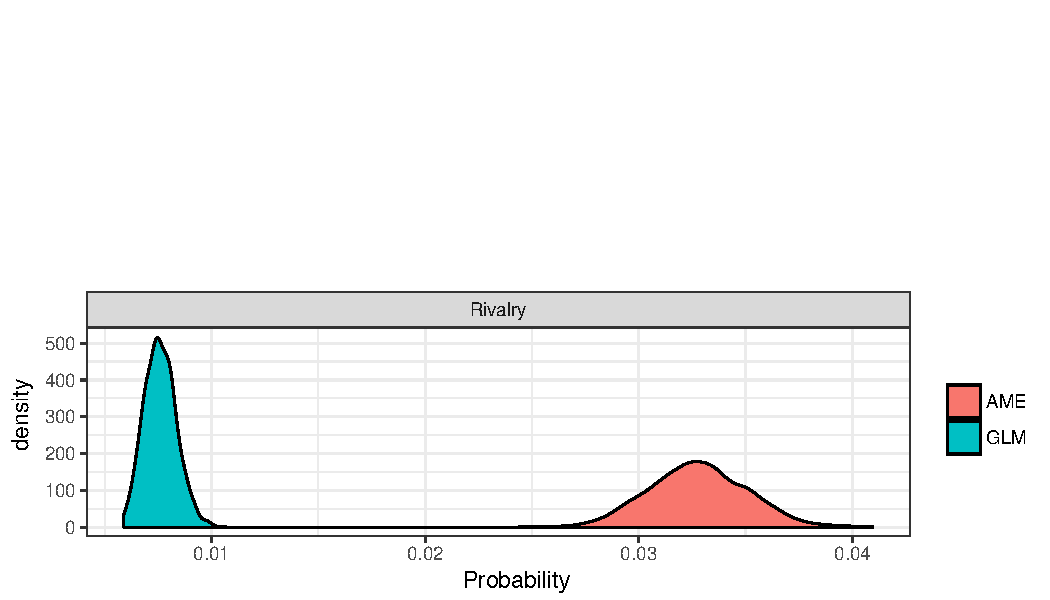
\includegraphics[width=\textwidth]{gibler_margeff.pdf}
 	\label{fig:gibmargeff}
 \end{figure}

We utilized the original and the AME results from Gibler's model 6 in Table 6 to calculate the expected values for one scenario focusing on the variables measuring rivalry.  We employed mean or modal values for all independent variables, except we changed the rivalry variable to indicate that there was a rivalry when the actual data suggest there is none.  The expected values of this scenario are essentially a first difference plot comparing results with the model when estimated in two different ways: Gibler's GLM estimation and our AME approach.  As this Figure~\ref{fig:gibmargeff} illustrates, the AME results differ notably. First, the expected value of the dependent variable---the probability of the onset of a militarized interstate dispute, is considerably lower when taking interdependencies into account with the AME model.  These are rare events, so the probabilities are low, but the difference is a factor of almost 2. Thus, you get quite substantially different expected values from these two models.  

\subsection{Lessons Learned from Re-estimating Five Prominent Studies}

First and foremost, many findings that emerge from models that do not take interdependencies into account lose their statistical significance when network effects are estimated via AME. Not only are coefficients biased in the GLM approaches to the analysis of dyadic data, but they are often imprecisely measured, with poorly calibrated standard errors.  This means that significance testing (for better or worse) is compromised when network effects are ignored.

Second, even when the results from the AME estimation conform with those found in an OLS or logistic regression, new insights emerge from the additional information derived. In particular, there is actual information about the dependencies so that clusters can be identified, and the extent of reciprocity at the dyad level, as well as among senders and receivers.  This kind of information is absent in standard approaches and adds to our ability to explain specific as well as general results.

Third, it is evident that the actual results---not the estimated coefficients and their covariances---which are generated by the models differ greatly in expectations.  This implies that policy experimentations with the models, as well as scenario-based simulations and forecasting of GLM models are likely to often give misleading results compared to the AME approach.

Fourth, it is clear that the AME approach dominates the GLM approaches in terms of performance. Not only it is better at correctly identifying cases in which the dependent variable takes a value of $0$ (via the ROC curves and associated statistics), but it also dominates at correctly identifying occurrences of the dependent variable in the data (seen via the PR curves and associated statistics).  In the case of studies with continuous dependent variables, the AME approach has average error statistics that are about one-half that found in the OLS model. 